Dieses Kapitel befasst sich mit der Implementierung eines Loggers, welcher firmenintere Daten der Firma FlexSolution möglichst effizient abspeichern soll, der Fokus liegt dabei bei der Performance. Daraufhin sollen die Werte fundiert in einem WebInterface dargestellt werden.

\begin{spacing}{1}
    \section{Untersuchungsanliegen}\label{section:untersuchungsanliegenFlexlogger}
    \end{spacing}
Das ist ein Test, um zu schaun, ob es so funktioniert, wie ich mir das vorstelle

\begin{spacing}{1}
    \section{IST-Stand}\label{section:ist-standFlexlogger}
    \end{spacing}
Die Firma FlexSolution befindet sich in der Lage, die benötigten Daten zu loggen (abzuspeichern) mithilfe von Log4J. Allerdings werden dabei die Daten zuerst in einer Datei gespeichert, darauffolgend komprimiert und in einem Ordner abgelegt. Nachdem diese Daten komprimiert wurden, gibt es nur sehr umständliche Möglichkeiten, die Daten auszulesen, da diese nicht zentral abgespeichert werden und ein Zugriff auf die Daten sich somit als sehr umständlich erweist. Das Ziel dieses Teils der Diplomarbeit ist, die Daten in Echtzeit zu loggen und in einer zusätzlichen Datenbank abzuspeichern, um diese anschließend grafisch ansprechend darzustellen.
 
\subsection{Log4J}
Framework, um Anwendungsmeldungen von JAVA zu loggen.


\begin{spacing}{1}
    \section{Aufbau des Projektes}\label{section:aufbaudesProjektesFlexlogger}
    \end{spacing}
\subsection{Beschreibung der Funktionen}
%% sehr einfache Beschreibung der Website mit vielen Screenshots von de einzelnen Komponenten (Button/ EinagbeFeld / was wird wann angezeigt etc.)


\subsection{Logger}
Das sogenannte FS-Logger-Programm setzt sich aus mehreren Klassen zusammen, wie etwa einen DataJDBCAdapter, einer Hauptklasse namens FlexTaskFsLogger. Weiteres befindet sich in dem Programm eine Modelklasse namens LogEntry, welche die Attribute der eingetragenen LogEntries definiert. Um die einen reibungslosen Ablauf zu garantieren, wird eine Blocking-Queue verwendet, welche Multithreading unterstützt. Das ganze Programm baut auf dem Producer Consumer Pattern auf.	

\subsubsection{DataJDBCAdapter}
Der DataJDBCAdapter ist dafür verantwortlich, eine Verbindung zu der PostgreSQL-Datenbank aufzubauen und somit die benötigten Objekte in einer Datenbank abzuspeichern (insert). Um diese Verbindung herzustellen, verwendet der JDBCAdapter eine URL, welche in einem String abgespeichert ist, sowie einen Usernamen und ein Passwort. Innerhalb der connect-Methode werden diese Daten verwendet, sie gibt ein Connection Objekt zurück, welches angibt, ob die Verbindung zur Datenbank erfolgreich war. Die connect-Methode wird innerhalb der darunterliegenden insertLogEntry-Methode aufgerufen. Wenn die Anbindung erfolgreich war, wird ein PreparedStatement mithilfe des vorher übergebenen SQL-String erstellt und darauffolgend ausgeführt. Somit wird erfolgreich ein neuer Datenbankeintrag in der Datenbank gespeichert. Falls während des ganzen Ablaufes ein unerwarteter Fehler auftauchen sollte, wird dieser mittels einer Java-Exception in die Konsole geschrieben.

\subsubsection{Main Klasse FlexTaskFsLogger}
Die Klasse FlexTaskFsLogger ist die Main-Klasse des Programms. Sie führt das Programm aus. Dieser Klasse werden auch folgende Methoden vererbt, da sie eine Subklasse der Klasse FlexTask ist: 
\begin{compactitem}
    \item getNeededTaskParameters
    \item getNeededDeviceParameters
    \item isSingleDeviceTask
    \item closing
    \item initTask
\end{compactitem}

Zusätzlich befindet sich noch in der Klasse eine Getter- und Setter-Methode, diese sind allerdings lediglich für eine Zählvariable zuständig, um bestimmte Daten weniger oft in die Datenbank einzuspeichern.

Das Haupmethode des FlexTaskFsLogger ist die initTask-Methode. In ihr wird eine BlockingQueue mit dem generic Type LogEntry erstellt. Mithilfe dieser Blocking-Queue wird darauffolgend ein Producer und ein Consumer erstellt, welche die Blocking-Queue als Parameter übergeben bekommen. Nachfolgend werden jeweils zwei Producer-Threads und zwei Consumer-Threads erstellt und gestartet. Um eine zeitliche Einteilung zu haben, wird ein sogenannter TimerTask erstellt, welcher wiederum auch ein neuer, unabhängiger Thread ist. Er wird dazu genutzt, um in einem gewissen Intervall Methoden oder Code-Blöcke aufzurufen. In diesem Fall wird der Task dazu verwendet, über den DataJDBCAdapter einen neuen Eintrag in die Datenbank zu speichern. Dazu wird zuallererst überprüft, ob eine Variable, welche für das Starten und Stoppen des Tasks zuständig ist, auf true gesetzt wurde. Anschließend wird ein sogenannter StringBuilder, welcher aus einer Kette von Strings besteht, aus dem vorher erstellten Consumer geholt. Dieser StringBuilder besteht aus einem aneinandergeketteten Insert-Statement. Um die Ausführbarkeit des Stringbuilders zu gewährleisten, muss die letzte Stelle (an welcher sich ein Beistrich befindet) gelöscht werden und durch einen Strichpunkt ersetzt werden. 

Um das korrekt erstellte SQL-Statement nun ausführen zu können, wird in einem try and catch Statement die insertLogEntry-Methode des DataJDBCAdapter ausgeführt. Dabei wird der StringBuilder mit dem SQL-Statement, welche mithilfe der toString-Methode in einen String umgewandelt wird, übergeben. 

Anschließend wird der eben verwendetet StringBuilder geleert, indem die delete-Methode aufgerufen wird. Um einen neuen Insert-Aufruf zu ermöglichen, wird ein insert-Header (siehe Abb.1) über die setStringBuilder-Methode aus dem Consumer gesetzt. 

Nun wird der vorher beschriebene TimerTask in einem eine Zeile davor erstellten Timer als Parameter übergeben.

Der nächste Abschnitt sorgt dafür, dass man das Programm, also den Consumer und Producer aus- und einschalten kann. Dazu werden zuerst zwei Datenpunkte initialisiert. Diese werden durch das Setzen einer spezifischen Adresse und dem Namen eines Datenpunkts erstellt. Dabei ist der Datenpunkt \texttt{logger\_nav\_status\_icon\_Click} dazu verantwortlich, darauf zu hören, ob sich ein Wert, welcher in diesen Datenpunkt gespeichert ist, geändert hat. Das heißt, wenn auf der eigens dafür erstellten Website der Ein- und Ausschaltknopf gedrückt wird, wird der Timer pausiert und das Programm schreibt keine Werte mehr in die Datenbank. Im Gegensatz dazu ist der \texttt{logger\_nav\_status\_icon\_State} dafür da, einen Wert für die Website zu übergeben. Damit wird die Farbe des Icons verändert, um dem User ein Feedback zu seiner Aktion zu geben.
Nachdem die Methode setDatapointChangedCommand mit dem \texttt{logger\_nav\_status\_icon\_Click} verbunden wird, wird aktiv auf den Datenpunkt gehört. Ein neuer DatapointCommand wird dabei übergeben, in ihm wird die execute-Methode überschrieben. In dieser Methode wird zuallererst eine temporäre Variable erhöht, sie ist dafür da jeden zweiten Dateneintrag zu überspringen, da die HMI jedes Mal zwei Werte schickt, allerdings nur einer benötigt wird. In Folge darauf wird in einem If-Statement der Wert des \texttt{logger\_nav\_status\_icon\_State} Datenpunkts geändert, um die Farbe des Einschalt Icons zu verändern. Zusätzlich wird die startOrStop Variable auf false gesetzt und der Producer und der Consumer werden mithilfe der Übergabe von ‚false‘ in der setRun-Methode gestoppt. Im else-Zweig des If-Statement wird genau das gegenteilige bewirkt, d.h. Producer und Consumer werden gestartet und die \texttt{logger\_nav\_status\_icon\_State} wird wieder auf den ursprünglichen Wert geändert. 

\subsubsection{LogEntry Klasse}
Dies ist die Model-Klasse des Programms. In ihr werden die Attribute des LogEntries festgelegt. Diese beinhalten die dp-id, d.h. die Id des Datenpunktes, welcher gespeichert werden soll. Außerdem wird der Wert des Datenpunktes, die Einheit und der Timestamp, also den genauen Zeitpunkt, an welchem der LogEntry erstellt wurde, angelegt. In der Klasse befinden sich zusätzlich Getter und Setter für die Attribute und ein Konstruktor. 

\subsubsection{Blocking Queue - Producer }
Diese Klasse ist der Producer der Blocking Queue, d.h. in dieser Klasse werden die Objekte in die Blocking Queue hinzugefügt. 

Es lassen sich zwei Attribute im Producer finden, die Blocking Queue, in welche die Objekte später hinzugefügt werden und eine Boolean Variable, welche den Namen “run” trägt. Sie ist dafür verantwortlich, den Producer zu deaktivieren bzw. zu aktivieren. Unterhalb der Attribute befinden sich ein Konstruktor, um die Blocking-Queue zu übergeben und ein Getter und ein Setter für die run-Variable. 

Die Hauptmethode der Klasse ist die run-Methode. Hier wird ein neuer DatapointCommand erstellt, in welchem die execute-Methode überschrieben wird. Innerhalb der execute-Methode wird ganz oben eine Counter Variable initialisiert, sie ist dafür verantwortlich, bestimmte Daten von Datenpunkte nur jedes zweite Mal in die Blocking Queue hinzuzufügen. Danach befindet sich ein if-Statement, welches überprüft, ob der Code im Consumer ausgeführt werden soll oder nicht. In diesem if-Statement befindet sich ein Switch für den specificDataType, welcher je nach DataType einen bestimmten Codeteil ausführt. In dem einen Codeteil wird die counter-Variable auf true oder false überprüft (bei einem false wird der Datenteil nicht in die Blocking-Queue hinzugefügt), in dem anderen wird dies ignoriert.

Allerdings kümmern sich beide Codeteile darum, die jeweiligen Daten als LogEntry zu erstellen und diesen anschließend in die Blocking Queue zu pushen.

Mithilfe des Codes, welcher sich unterhalb des erstellten DataPointCommands befindet, wird über die Datenpunkte des jeweiligen Geräts iteriert und sorgt dafür, dass der oben liegende Codeteil bei einer Änderung ausgeführt wird.  

\subsubsection{Blocking Queue - Consumer }
In dieser Klasse geht es um den Consumer der Blocking Queue, d.h. vom Consumer werden Objekte aus der Blocking Queue genommen und diese weiterverarbeitet. Die Attribute in dieser Klasse sind so wie in der Producer Klasse eine Blocking-Queue, sowie die run-Variable, um den Consumer zu aktivieren bzw. zu deaktivieren. Im Konstruktor wird wiederum die Blocking-Queue übergeben.

In der run-Methode der Klasse wird in einem while-True ein if-Statement ausgeführt, in welchem sich ein try- and catch-Statement befindet. In diesem wird das benötigte Objekt aus der Blocking-Queue geholt und anschließend in einen StringBuilder als gültiges SQL-Statement hinzugefügt.

Unterhalb befindet sich noch eine Getter- und Setter-Methode für den StringBuilder sowie die run-Variable.

\subsection{Quarkus Backend (Beschreibend)}
Das Backend besteht aus JAVA und dem Java-Framework Quarkus. 

\subsubsection{LogEntry Klasse}
Hier werden die Attribute des LogEntries festgelegt. Diese beinhalten wie auch im Programm FlexTaskFsLogger die dp-id, den Wert, die Einheit und einen aktuellen timestamp des Eintrags. 
Auch beinhaltet ist ein Konstruktor, Getter- und Setter-Methoden für die Attribute sowie eine toString-Methode, um die Attribute formatiert zurückgeben zu können. 

\subsubsection{LogEntry Ressource}
Mithilfe dieser Klasse werden bestimmte Daten an bestimmte vorher definierte Adressen geschickt. 
Der vorher definierte Path ‚/logEntry‘ wird dabei bei jeder Anfrage am Anfang der Adresse verwendet. 
Um das davor erstellte LogEntry Repository zu verwenden, wird es am Anfang der Methode mit dem Schlüsselwort new initialisiert.

In der Ressource befinden sich verschiedenste GET-Methoden, welche alle einen anderen Nutzen haben: 

\begin{compactitem}
    \item getAll(): Hier wird durch die Übergabe der Parameter definiert, in welchem Zeitraum die benötigten Daten zurückgegeben werden. Diese Parameter werden mithilfe von PathParam übergeben, d.h. die Daten werden über die URL übergeben. Zusätzlich steht über der Methode ein \texttt{@Produces(MediaType.APPLICATION\_JSON)}, um festzulegen in welchem Format der Rückgabewert zurückgeben wird. In diesem Fall ist es das JSON-Format.
    \item getByName(): Diese Methode ist sehr ähnlich zur getAll()-Methode. Lediglich wird ein zusätzlicher Name übergeben und somit die getByName-Methode des Repositories verwendet. 
    \item getCSV(): In dieser Methode wird im Pfad neben den Daten ein filePath angegeben, in welchem die CSV-Datei gespeichert werden soll. Mithilfe der getCSVAll-Methode aus dem Repository wird die CSV-Datei anschließend im richtigen Pfad gespeichert. 
    \item getCSVByName(): Die Methode hat eine ähnliche Funktion wie die getCSV()-Methode. Der entscheidende Punkt dabei ist, dass ein Name übergeben werden kann, welcher die Rückgabedaten beeinflusst, da so nur die Daten mit dem richtigen Namen als CSV-Datei erstellt wird.  
    \item insert(): Mithilfe dieser Methode kann ein neuer LogEntry in die Datenbank eingefügt werden. Als Parameter in der insertLogEntry-Methode des Repositories wird dabei ein neu erstellter LogEntry übergeben.
    \item downloadFile(): Um das vorher erstellte CSV-File zu downloaden, wird diese Methode genutzt. In diesem Fall ist der Rückgabewert der Methode mit einem \texttt{@Produces(\{"text/csv"\})}definiert, da es sich dabei um eine CSV-Datei handelt. Zuallererst wird in der Methode ein File-Name, ein Pfad, sowie ein File erstellt. Der Pfad und der File-Name ist dabei jeweils vom Datentyp String, das File ist vom Datentyp File und wird mithilfe des Pfads als Parameter erstellt. Um zu überprüfen, dass der Pfad existiert, wird mithilfe eines IF-Statements die Methode exists() beim vorher erstellten File als Übeprüfung herangezogen. Wenn dieses IF-Statement feststellt, dass das File nicht existiert, wird eine RuntimeExcpetiion geworfen. Diese enthält die Nachricht "File not found: " und den zugehörigen File-Namen. Bei einem erfolgreichen erstellen des Files wird ein ResponseBuilder namens res erstellt. Dieser enthält die Resonse OK sowie das File. Zusätzlich wird bei dem ResponseBuilder ein Header gesetzt, in welchem sich unter anderem der FileName befindet. Schlussendlich wird der ResponseBuilder mit einem Build-Statement zurückgegeben.  Somit wurde das vorher erstellte File erfolgreich heruntergeladen und kann nun mithilfe von einem passenden Programm geöffnet und gesichtet werden.
\end{compactitem}

\subsubsection{LogEntry Repository}
Das Repository des Backends ist dafür verantwortlich, eine Verbindung zur Datenbank herzustellen und die richtigen Daten an die Ressource weiterzugeben. Zuallererst werden drei verschiedene Strings definiert, um Zugriff auf die Datenbank zu erlangen. Der erste ist dabei die URL, um sich zur Postgres-Datenbank zu verbinden. Der zweite und dritte String definiert den User sowie das Passwort, um Zugriff zur Datenbank zu erlangen. 

Die erste Methode in der Klasse trägt den Namen connect. Wie der Name schon sagt, wird in der Methode mithilfe eines DriverManagers wird eine Verbindung zur Datenbank aufgebaut und zurückgegeben, welche in den folgenden Methoden verwendet werden kann. 

\begin{lstlisting}[language=java,caption=Connect to SQL Database,label=lst:impl:connect]
    /**
    * Connect to the PostgreSQL database
    *
    * @return a Connection object
    */
   public Connection connect() throws SQLException {
       return DriverManager.getConnection(url, user, password);
   }   
\end{lstlisting}

Jede der nachfolgenden Methoden ist für eine bestimmte Aktion auf der Datenbank zuständig. 
Um alle vorhandenen LogEntrys in einem bestimmten Datums-Bereich zu erlangen, kann die getAll-Methode verwendet werden. Die übergebenen Parameter sind dabei das Anfangs- und das Enddatum, sowie die Anfangs- und die Endzeit. Anfangs wird nun ein Set von logEntries erstellt, in welchem nachfolgend die Daten hinzugefügt werden. Um das Datum und die Zeit in Millisekunden umwandeln zu können, da nur diese später in einem SQL-Statement verwendet werden können, wird eine convertToMillis-Methode verwendet. So wird eine Start- und Endzeit in Millisekunden erstellt. 
Um die Daten, welche zwischen dem Start- und dem Enddatum liegen, zu bekommen wird in einem SQL-Statement definiert, dass der timestamp des jeweiligen LogEntries größer als die Startmillisekunden, und kleiner als die Endmillisekunden ist. Außerdem werden die Daten nach dem timestamp geordnet. Anschließend wird eine Verbindung zur Datenbank aufgebaut. Um das vorher erstellte SQL-Statement nutzen zu können, wird ein PreparedStatement genutzt. In diesem werden die beiden Parameter startMilllis und endMillis gesetzt. Aus diesem PreparedStatement wird nun ein ResultSet gewonnen, durch die Methode executeQuery. Um vollständige LogEntries zu erhalten, werden alle ResultSets mithilfe einer while-Schleife durchgegangen. Jeder der LogEntries wird zu dem Set namens logEntries hinzugefügt. Um die richtigen Spalten der logEntries zu bekommen, wird der Name der Spalte verwendet. 

Bei einem Fehler in der Verbindung zur Datenbank wird eine Fehlermeldung ausgegeben. Bei einem Erflog wird das Set von LogEntries zurückgegeben und kann somit in der Ressource verwendet werden. 

Die getByName-Methode ist sehr ähnlich zur getAll-Methode. Der einzige Unterschied ist, dass als Parameter zusätzlich ein Name mitübergeben wird. Dieser wird zusätzlich im SQL-Statement gesetzt und somit werden alle LogEntries, welche einen anderen Namen tragen aussortiert. Zurückgegeben wird erneut ein Set aus LogEntries.

Die bereits verwendete convertToMillis-Methode befindet sich direkt unter der vorigen Methode. In ihr wird das Datum und die Zeit als gemeinsamer String erstellt. Dieser String wird nun verwendet, um eine Variable des Typs LocalDateTime zu erstellen. Dieses wird nach dem richtigen Formatieren bzw. Umwandeln zurückgegeben.

Der nächste Abschnitt des Repositories ist für alle Methoden rund um das Erstellen von CSV-Dateien zuständig. Die ersten beiden Methoden unterteilen jeweils, ob ein Name mitübergeben wurde, oder nicht. Die Parameter sind dabei das Anfangs- und Enddatum, sowie die Anfangs- und Endzeit. Bei der zweiten Methode wird nun ein Name zusätzlich übergeben. Der meiste Teil der Methoden ist relativ ähnlich, zuerst wird ein Set von LogEntries erstellt. Je nach Methode werden mithilfe der Parameter die richtigen logEntries mit der getByName-Methode bzw. der getAll-Methode  in dem Set gespeichert. Nachfolgend wird aus dem Set ein Stream erstellt, dabei wird jedes logEntry-Objekt zu einem String umgewandelt. Anschließend wird jeweils die Methode writeToCSVFile aufgerufen, welche sich direkt unter den anderen zwei Methoden befindet. Übergeben wird dabei beide Mal der zuvor erstellte Stream mit den Strings, sowie ein neu erstelltes File mit einem vorher erstellen FilePath. 

Die erste Zeile in der writeToCSVFile-Methode konvertiert das eben übergebene Set zu einer Liste. In diesem Prozess wird eine weitere Methode angewendet, welche den Namen convertToCSVFormat trägt. Mithilfe eines map-Befehls wird die Methode auf jeder Zeile des Sets angewendet. Die convertToCSVFormat-Methode gibt dabei die übergebene Zeile als Stream zurück, wobei zwischen den einzelnen Werten in einer Zeile ein Semikolon eingefügt wird. Als nächstes wird ein BufferedWriter verwendet. Dieser wird als neue Instanz erstellt, mit dem Übergabeparameter eines neuen FileWriters, in welchem das am Kopf der Methode übergebene File übergeben wird. Der BufferedWriter ist von einem Try- and Catch umgeben. Dies ist erforderlich, um bei einem eventuell auftretenden Fehler, wie etwa einem falschen Filepath oder fehlenden Berechtigungen, mit einer Fehlermeldung richtig reagieren zu können. In diesem Try- and Catch wird nun jede Zeile der vorher erstellten Liste mithilfe einer For-Schleife durchgegangen. Mit den Methoden write() und newLine() wird somit die CSV-Datei Zeile für Zeile erstellt. 

Die letzte Methode im Repository ist die insertLogEntry-Methode. Wie der Name bereits verrät, ist sie dafür zuständig, neue LogEntries in der Datenbank zu speichern. Um einen neuen LogEntry zu speichern, wird zuallererst ein String erstellt, welcher ein Insert-Statement enthält, erstellt. 
Danach wird eine Verbindung zur Datenbank mithilfe der connect-Methode hergestellt. Durch ein PreparedStatement, welches aus SQL-String geformt wird, könne alle Parameter gesetzt werden. Diese beinhalten die dpId (der Name des Datenpunkts), die value (den Wert des Datenpunkts), die unit (die Einheit des Datenpunkts), sowie den timestamp (wann der Datenpunkt erstellt wurde). Nachdem alle Parameter gesetzt wurden, wird ein executeUpdate durchgeführt, mithilfe dessen der neue LogEntry in die Datenbank geschrieben wird. 

\subsection{Angular Frontend (Beschreibend)}
\subsubsection{Website Ansicht}
Die erste Seite, welche man betritt, wenn man das Programm startet, ist die Hauptseite \ref{fig:impl:FlexLoggerHauptseitenAnsicht}. Auf ihr findet man 3 verschiedene Formulare. Jedes dieser Formulare hat eine andere Funktion. Das erste ist dafür zuständig, alle Diagramme in einem bestimmten Zeitraum anzuzeigen. Wenn man den Button dieses Formulars betätigt, wird man auf eine Seite weitergeleitet. Auf dieser kann nun zwischen allen Diagrammen mithilfe von Buttons wechseln \ref{fig:impl:FlexLoggerDiagrammAnsicht}. Das zweite Formular hat eine ähnliche Funktion. Lediglich kann man hier das Diagramm, welches man angezeigt bekommen will, im Formular mitübergeben. Durch den Button wird man nun direkt zum gewünschten Diagramm weitergeleitet. 

Eine ganz andere Funktion hat das letzte Formular. In ihm wird zwar genauso der Wunschzeitraum angegeben, allerdings wird nach Betätigen des Buttons ein CSV-File generiert und anschließend gedownloadet. In diesem werden alle Daten übersichtlich angezeigt. 



\begin{figure}
    \centering
    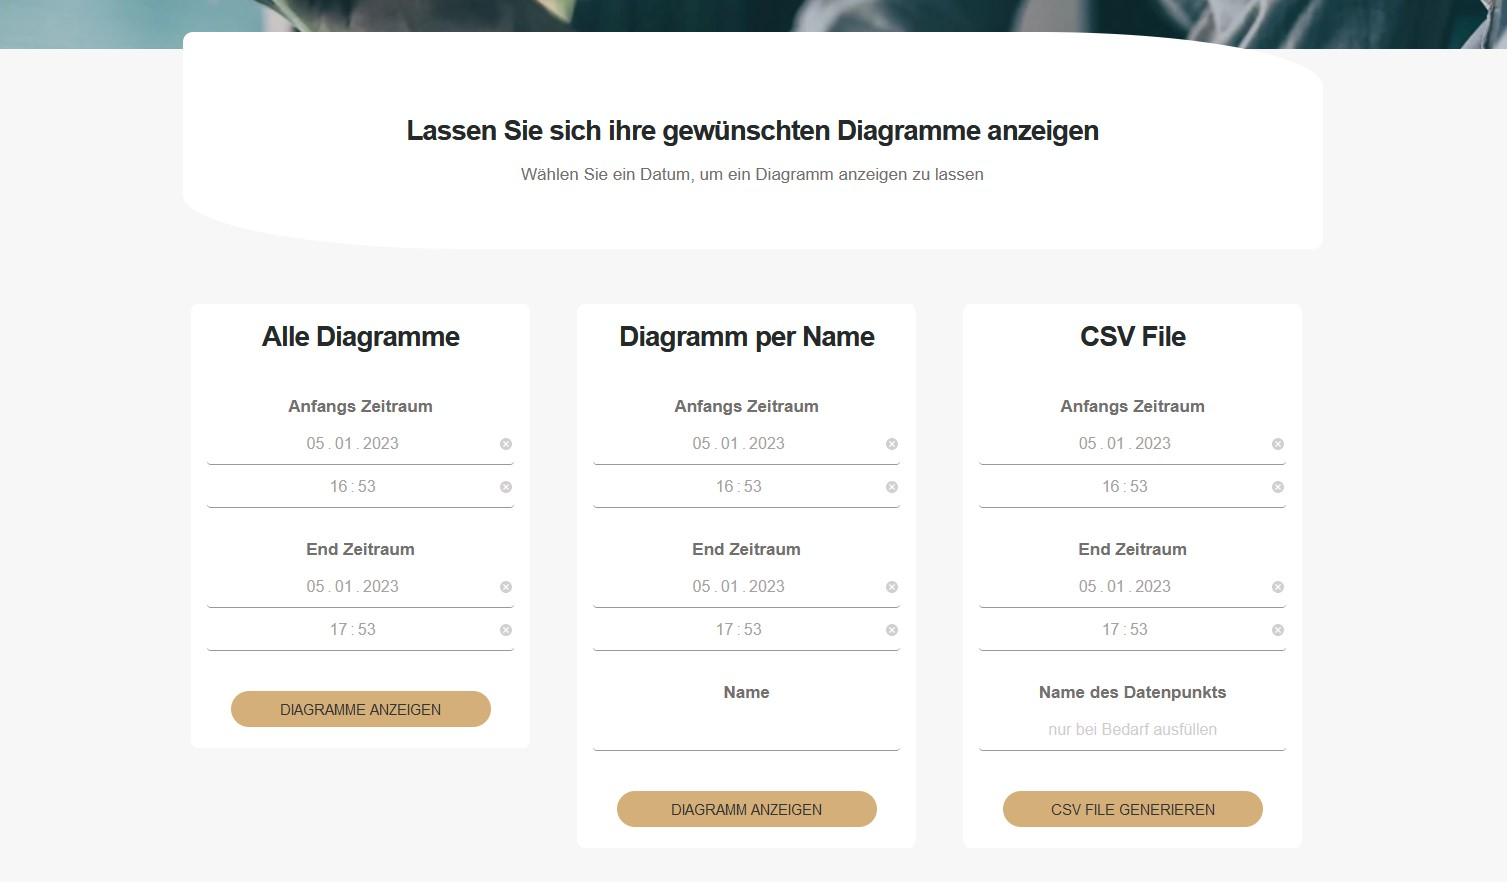
\includegraphics[scale=0.45]{pics/FlexLoggerWebsiteFormulare.jpg}
    \caption{Website Hauptseitenansicht}
    \label{fig:impl:FlexLoggerHauptseitenAnsicht}
\end{figure}

\begin{figure}
    \centering
    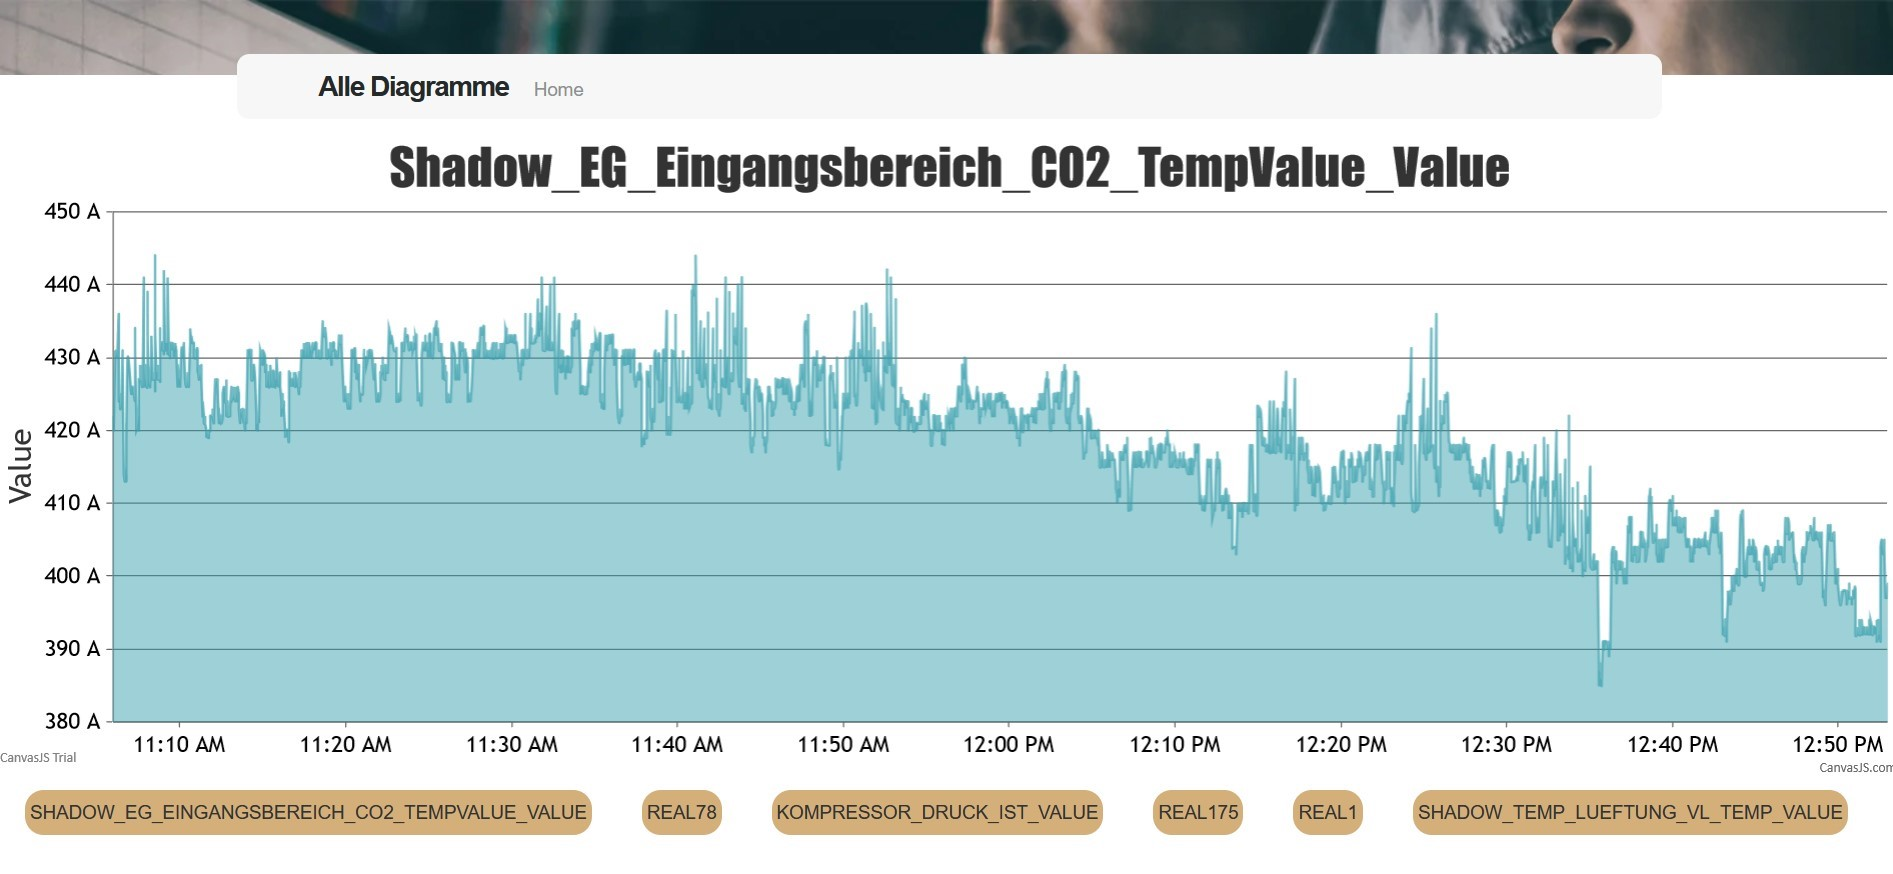
\includegraphics[scale=0.35]{pics/FlexLoggerWebsiteDiagramm.jpg}
    \caption{Website Diagrammansicht}
    \label{fig:impl:FlexLoggerDiagrammAnsicht}
\end{figure}

\subsubsection{App-Component}
In der TypeScript Klasse der App-Komponente wird ansich ein Titel definiert, dieser trägt in diesem Fall den Namen „flexloggerFE2“. Im HTML-File ist dabei ein Router-Outlet definiert. Durch dieses wird das Routing im Projekt ermöglicht. Das heißt jede Komponente wird praktisch in der App-Komponente angezeigt. In der app-routing-module Klasse werden alle Pfade des Projekts definiert. Dabei wird jeweils ein String als Pfad angeben, sowie eine Komponente definiert, zu welcher der Pfad führen soll. Zusätzlich wird bei den Modulen des Projekts ein RouterModule hinzugefügt, welches zusätzlich die Methode forRoot verwendet, in welchem die vorher definierten Routen als Parameter übergeben werden. In der app-module Klasse werden noch weitere Module hinzugefügt: 

\begin{compactitem}
    \item BrowserModule: Stellt einen Service zur Verfügung, mit welchem man eine Browser-app starten, sowie laufen lassen kann.    
    \item AppRoutingModule: Ermöglicht das Navigieren zwischen verschiedenen Komponenten.     
    \item HttpClientModule: Mithilfe dieses Moduls können Netzwerk Requests abgesetzt werden. Diese inkludieren GET, POST, PUT, PATCH und DELETE.    
    \item FormsModule: Durch dieses Modul können template-driven Forms erstellt werden.    
    \item ReactiveFormsModule: Mithilfe dieses Moduls kann ein reactiveForm verwenden. 
\end{compactitem}

\subsubsection{Home-Component}
Die ist die Haupt Komponente des Programms. In ihr werden 3 Formulare definiert, jedes davon hat eine andere Funktion. Im Konstruktor der Komponente werden verschiedenste Parameter übergeben:

\begin{compactitem}
    \item HttpService: Dies ist der Service, mithilfe dessen eine Server-Verbindung zum Backend aufgebaut werden kann.    
    \item Router: Mithilfe dieses in Angular eingebauten Features kann auf der Website zwischen den Komponenten gewechselt werden.        
    \item ActivatedRoute: Mithilfe dieses Parameters können Daten über Komponenten hinweg übergeben werden.    
    \item FormBuilder: Durch diesen Parameter können Reactive Formulare erstellt werden??
    \item ValidatorService: Wird später verwendet, um die Richtigkeit der Eingabe bei den Formularen zu garantieren.
\end{compactitem}

Im Konstruktor selbst, wird das heutige Datum sowie das heutige Datum plus einer Stunde gesetzt.
Um die Komponente zu initialisieren, wird in der ngOnInit()-Methode die initForms-Methode aufgerufen. Diese initialisiert alle 3 Formulare, indem sie die Variablen in den Formularen, sowie Validatoren setzt. Dabei werden bei den Variablen jeweils ein Standard-Wert gesetzt. Die gesetzten Validatoren überprüfen dabei, ob die Daten korrekte Eingaben in den Formularen sind. 

Weiteres findet man in der Komponente zwei Methoden, welche sich um das Routing kümmern. Diese kommen beim Klicken der Buttons der Formulare zum Einsatz, um die Komponente, welche angezeigt wird, zu wechseln. Die benötigten Daten werden dabei in der URL übergeben.

Die nachfolgende Methode ist für das Generieren sowie das Downloaden einer CSV-Datei zuständig. Zuallererst wird die checkCSV-Methode aufgerufen, in welcher überprüft wird, ob in dem ausgewählten Zeitraum Daten verfügbar sind.

Wenn die checkCSV-Variable als true gesetzt wurde, wird überprüft, ob der Namenparameter im Formular nicht leer ist. Trifft dies ein, wird mithilfe eines Timers und des Http-Service eine CSV-Datei generiert, welche alle Datenpunkte in dem richtigen Datumsbereich generiert. Nachdem das Generieren erfolgreich abgeschlossen wurde, wird der Download der Datei gestartet. Dieser Download wird mithilfe der window.open() Methode verwirklicht. Wenn der Namenparameter in dem Formular einen Namen enthält, so wird ein CSV-File generiert, welches nur die Daten eines Datenpunkts beinhält.

Wenn der Fall eintrifft, dass die checkCSV-Variable auf false gesetzt wurde, dann werden die Errors des Namenparameters auf true gesetzt. Dadurch wird unter dem Formular eine Fehlermeldung ausgegeben, um dem User eine Rückmeldung der Formulareingabe zu geben.

\subsubsection{Canvas-Chart-Component}

In dieser Komponente wird ein Diagramm erstellt, in welchem anschließend mithilfe von verschiedenen Buttons die gewünschten Daten angezeigt werden.  

Der erste wichtige Teil der Komponente ist das Erstellen der Diagramm Optionen. In diesen kann man verschiedenste Attribute eines Diagramms definieren: 

\begin{compactitem}
    \item animationEnabled: Stellt ein, ob beim ersten Anzeigen eines Diagramms jeder Punkt des Diagramms flüssig geladen wird, um ein dynamischeres Ergebnis zu erhalten.    
    \item title: Setzt den Titel fest, welcher als Überschrift über dem Diagramm stehen soll.          
    \item axisY: Legt den Titel der Y-Achse fest, diese Einstellung kann genauso auf der X-Achse getätigt werden.    
    \item data: Dies ist die wichtigste Einstellung der Diagramm Optionen. Sie legt den Typ des Diagramms fest (in diesem Fall ist es ein Liniendiagramm), die Farbe des Diagramms und setzt die Datenpunkte fest. Beim ersten Laden der Seite werden die Datenpunkte der X- und Y- Achse auf 0 bzw. den 01.01.1970 gesetzt. 
\end{compactitem}

Beim Laden der Seite wird zuerst im Konstruktor der Komponente eine Funktion namens onload() ausgeführt. Diese ist dafür zuständig, die erforderlichen Daten mithilfe des http-Service aus dem Backend zu bekommen. Zuerst werden hierfür die übergebenen Werte aus dem Formular mithilfe von Route Snapshots übergeben. Anschließend wird durch den http-Service eine getLogEntries-Methode aufgerufen, diese gibt die Werte zurück, welche das erforderliche Datum besitzen. Diese werden nun in einem Array gespeichert, um weiter verwendet zu werden.

Ion der nächsten Zeile des Konstruktors befindet sich ein Timer, welcher nach 1? Sekunde den darauffolgenden Code durchführt. In diesem Code wird zuallererst eine getFiles-Methode ausgeführt, diese gibt das vorher erstellte Array zurück. Das IF-Statement eine Zeile darunter garantiert, dass die Länge des Arrays nicht 0 beträgt, ansonsten wird die Fehlermeldung "Zu Ihrem ausgewählten Zeitpunkt wurden keine Daten gefunden." ausgegeben. Bei einem positiven Ergebnis des IF-Statements werden nachfolgend vier Methoden aufgerufen: 

\begin{compactitem}
    \item getListOfDatapointNames(): Diese Methode kümmert sich darum, eine Liste der Namen für die Buttons zu erstellen. Diese Buttons sind später dafür zuständig, zwischen den angezeigten Daten zu wechseln. 
    Um zu verhindern, dass der Name eines Datenpunkts öfters in der Liste vorkommt, wird am Beginn eine Boolean-Variable namens nameInList erstellt. Diese wird vorerst auf False gesetzt.
    Anschließend wird ein vorher initialisiertes Array auf ein leeres Array gesetzt, in welches danach die Namen hinzugefügt werden. Um alle Namen aus den Daten zu erlangen, wird eine for-Schleife verwendet, welche alle vorher erhaltenen Daten durchgeht. Der erste Name wird immer hinzugefügt, daher wenn die Länge des leeren Arrays 0 ist, wird der erste name hinzugefügt. Sonst wird eine weitere for-Schleife betreten, welche alle Elemente der List der Namen durchgeht. Wenn ein Element bereits vorhanden ist, wird die nameInList Variable auf true gesetzt. Später wird in einem weiteren If-Statement überprüft, ob diese Variable auf True oder False gesetzt ist. Bei einem False wird dabei der Name in die Liste hinzugefügt. Durch dieses Verfahren wird sichergestellt, dass kein Name doppelt in der Liste vorkommt und somit Buttons nicht doppelt angezeigt werden.    
    \item changeData()
    Hier werden die geänderten Daten in die Diagramm Optionen gespeichert. Um dies umzusetzen, wird als Parameter ein String namens filterString übergeben. Mithilfe diesem und einer For-Schleife werden alle Datenpunkte herausgefiltert, welche nicht den gewünschten Namen besitzen. Die richtigen Daten werden nun im Array dynamicLogLines gespeichert. Nach dem Aussortieren der Daten wird mit einem IF-Statement überprüft, ob die erste Stelle des dynamicLogLines nicht undefiniert ist. Wenn dies der Fall ist, wird der erste Datenpunkt, sowie der Titel in den Diagramm Optionen gesetzt. Danach werden die restlichen Datenpunkte mithilfe einer For-Schleife in den Diagramm Optionen gespeichert.               
    \item setChartOptions()
    Beim Aufrufen dieser Methode werden die Diagramm Optionen neu gesetzt. In diesem Fall wird der Titel, die Einheit und die Datenpunkte des Diagramms erneuert.        
\end{compactitem}

Anschließend wird eine Boolean-Variable namens showChart auf True gesetzt, wenn dieser Fall eintritt, wird auf der Website ein Diagramm angezeigt. 

\subsubsection{Canvas-Chart-Single-Component}
Die Komponente ist vom Aufbau her sehr ähnlich wie die Canvas-Chart-Komponente. Genau wie in der anderen Komponente werden zuerst einige Methoden im Konstruktor aufgerufen. Der größte Unterschied dabei ist, dass keine Buttonnamen erstellt werden, bzw. auch keine Buttons angezeigt werden. 

\subsubsection{HttpService}
Der Service ist dafür zuständig, die jeweiligen Daten aus dem Backend zu beschaffen. Zuerst wird ein String definiert in welchem die URL des Backend gespeichert ist. Im Konstruktor wird der sogenannte HttpClient als Parameter übergeben, er ist der Hauptakteur in der Klasse. Mithilfe von ihm kann eine Verbindung zum Server hergestellt werden. 

In dem Service befinden sich mehrere Methoden. Allgemein kann man sagen, dass man mit dem HttpClient jeweils einen GET-Request absetzt, welcher jeweils ein anderes Ergebnis liefert, je nachdem welche URL man als Parameter übergibt.

Die ersten beiden haben jeweils als Rückgabe-Paramater ein LogEntry Array. Beide geben die gesuchten Daten in einem bestimmten Zeitraum zurück, lediglich kann man bei der zweiten Methode noch einen Namen hinzufügen. Die Daten, welche die Zeiträume definieren, werden als Parameter in den Methoden übergeben. Die nächsten Methoden sind allesamt für das Downloaden eines CSV-Files verantwortlich. Dabei kümmern sich die ersten beiden um das Erstellen der CSV-Datei, die dritte ist für den eigentlichen Download verantwortlich. Um die CSV-Datei zu erstellen, werden wiederum die gewünschten Daten übergeben und anschließend wird daraus eine URL gebaut und ein GET-Request abgesetzt. Der einzige Unterschied zwischen den Methoden ist abermals ein zusätzlicher Name-Parameter. Die downloadCSV-Methode verwendet wie die anderen Methoden einen GET-Request, allerdings hat sie den weiteren Parameter responseType. Dieser ist notwendig, da innerhalb des Requests eine CSV-Datei gedownloadet wird und somit der Response-Type Array-Buffer definiert werden muss. 

\subsubsection{ValidatorService}
Der ValidatorService ist dafür zuständig, die Richtigkeit der Eingabe im Formular zu überprüfen. Wenn diese als nicht akzeptabel erkannt wurden, werden die Errors der Parameter auf true gesetzt, und somit eine Fehlermeldung ausgegeben.

Die match-Methode überprüft ob jedes eingegebene Datum als valide Eingabe akzeptiert werden kann. Dabei werden zuerst alle Controls des Formulars übergeben. Bei der ersten Überprüfung handelt es sich darum, ob das Startdatum hinter dem Enddatum liegt. Bei Bestätigung dieser Überprüfung werden die Errors mit dem Namen dateMustBeBigger aktiviert. Anschließend wird der Fall überprüft, wenn die beiden Daten gleich sind, die Zeiten sich allerdings unterscheiden, d.h. der Zeitraum am gleichen Tag stattfindet. Dies ist grundsätzlich erlaubt allerdings nur, wenn die Startzeit kleiner ist als die Endzeit. Wenn dies nicht der Fall ist, wird der Error timeMustBeBigger aktiviert.

\subsubsection{LogEntry Model}
Hier wird ein Model erstellt, welches den Namen LogEntry trägt, in diesem werden die Parameter dpId, value, unit und timeStamp definiert. Das Model wird dazu verwendet, um die vorher geloggten Daten aus der Datenbank weiterzuverwenden. 

\subsection{CanvasJS}
Mithilfe von CanvasJS, welche eine HTML5 und Javascript Charting library ist, wird das Anzeigen der Daten in Diagrammen ermöglicht. 

\begin{spacing}{1}
    \section{Logging}\label{section:logging}
    \end{spacing}

% < 1 Big Data in der Praxis - Lösungen mit Hadoop, Spark, HBase und Hive. Daten speichern, aufbereiten, visualisieren. 2. erweiterte Auflage, von  Jonas Freiknecht, Stefan Papp, 2018, S
% < 1 https://www.omega.com/en-us/resources/data-loggers
% 0 https://www.researchgate.net/profile/Anne-Ojala/publication/254255682_Eddy_Covariance_A_Practical_Guide_to_Measurement_and_Data_Analysis/links/00b7d51fbaa83999a4000000/Eddy-Covariance-A-Practical-Guide-to-Measurement-and-Data-Analysis.pdf#page=80
Data Logging kann dazu verwendet werden, Code zu debuggen oder große Datenmengen zu speichern, um diese später auszuwerten. Im Allgemeinen ist ein Datalogger ein Instrument, welches Veränderungen unter bestimmten Bedingungen während einer gewissen Zeitspanne aufzeichnet. Ein Datenlogger verwendet häufig Sensoren, um Daten zu sammeln. Anschließend können die Daten ausgelesen, visuell dargestellt und/oder ausgewertet werden. Die Daten, welche von Datenloggern ausgelesen werden, sind meist Druck, Temperatur, Luftfeuchtigkeit, Spannung oder Stromstärke. \cite{DataLogging} 

Die gespeicherten (geloggten) Daten können zum Beispiel dazu verwendet werden, 

\begin{compactitem}
    \item um die Temperatur und die Luftfeuchtigkeit in einem Gebäude zu überprüfen
    \item Information zur Gebäudewartung zur Verfügung zu stellen, dies betrifft das Heizen, die Belüftung, wie die Klimatisierung. Diese ständige Überprüfung der Daten kann den Energieverbrauch reduzieren
    \item die Wachs-Bedingungen von Pflanzen in der Landwirtschaft zu beobachten
    \item die Impfstoff-Lagerung in medizinischen Einrichtungen zu überwachen
    \item die Temperatur von Lebensmittel zu überprüfen
\end{compactitem}
\cite{DataLogging}

Logging bieten eine große Flexibilität und eignet sich gut, um große Datenmengen zu erfassen und auszuwerten. \cite{BigDataBuch}

\subsection{Loggen der Daten in der Firma}
Um die Daten zu loggen, also abzuspeichern, werden diese aus sogenannten Datenpunkten aus der firmentinternen FlexCloud ausgelesen. Diese werden angesprochen und aus ihnen kann dann der aktuelle Wert des Datenpunkts ausgelesen werden, siehe \ref{fig:impl:datenlogging}.
Beispiele für Datenpunkte der Firma FlexSolution, die ausgelesen werden: 

\begin{compactitem}
    \item Daten der Ladestationen
    \item Daten der Photovoltaik-Anlage am Dach
    \item die Temperatur in den Firmengebäuden
    \item Kompressor-Druck von Maschinen
    \item weitere Maschinendaten
\end{compactitem}

\begin{figure}[h t]
    \centering
    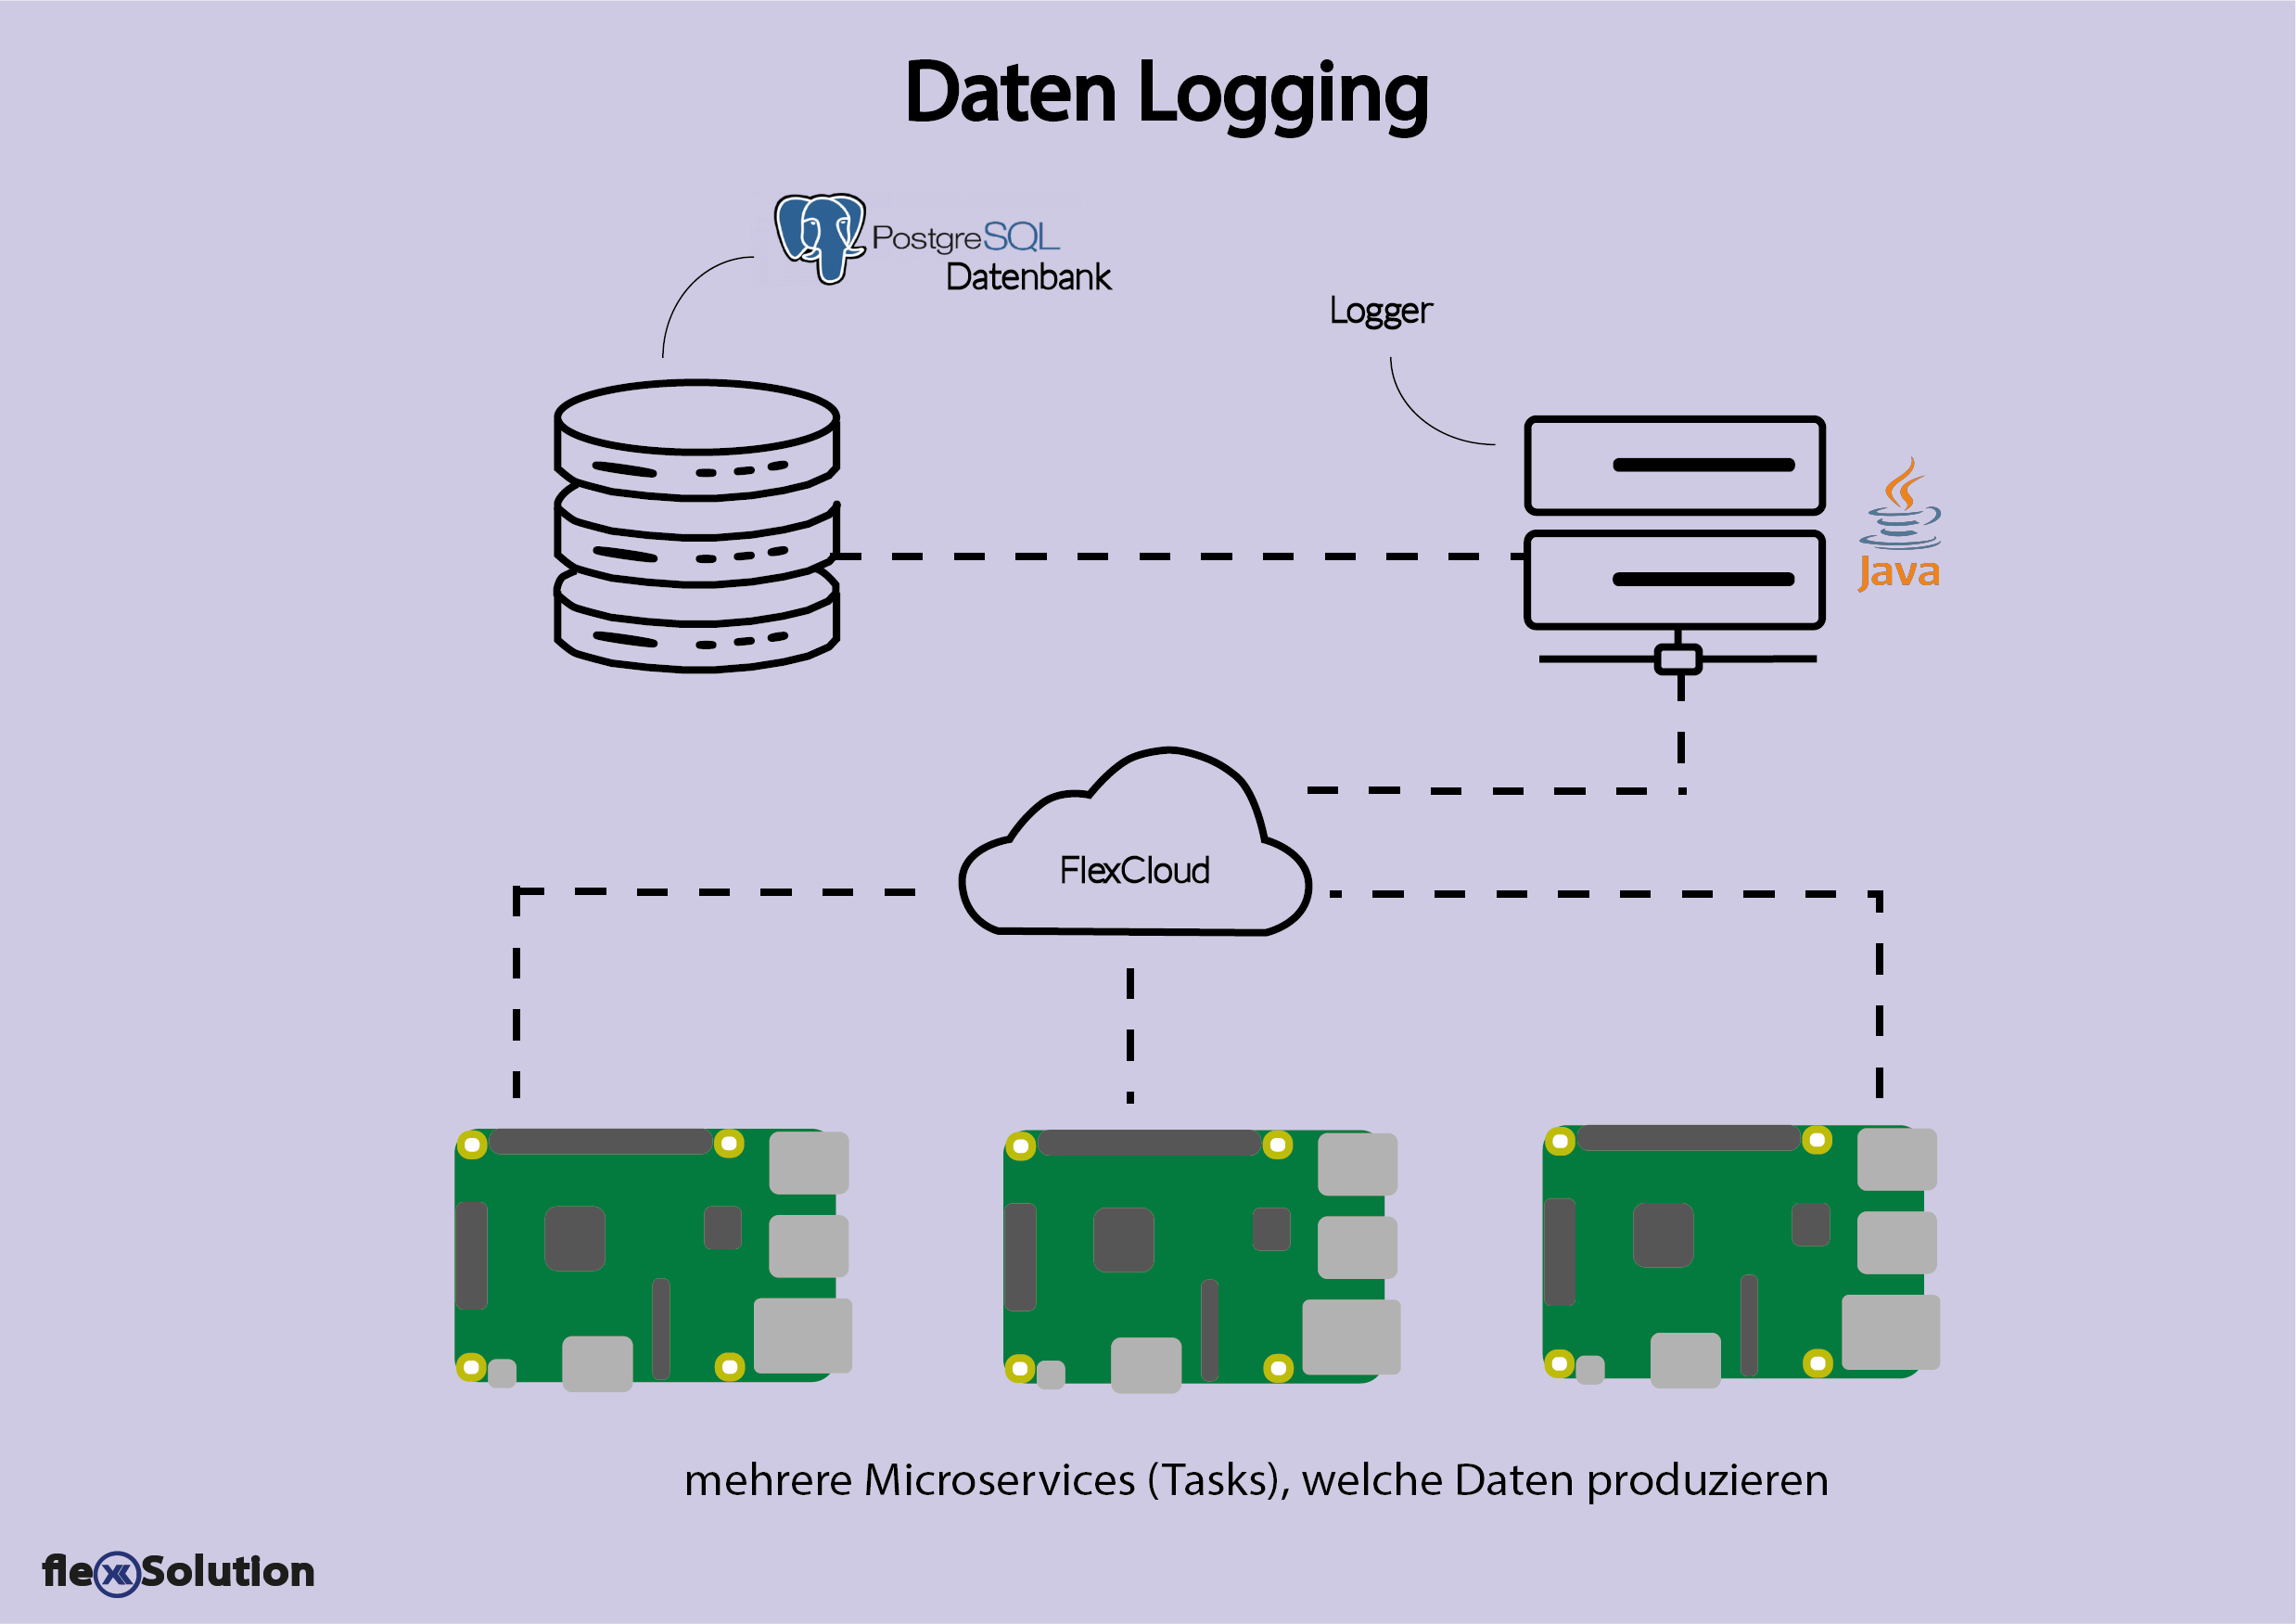
\includegraphics[scale=0.7]{pics/datenlogging.png}
    \caption{Daten Logging}
    \label{fig:impl:datenlogging}
\end{figure}

Das Logging-Programm wird mithilfe des Terminals gestartet. Sobald dieses gestartet wurde, siehe \ref{fig:impl:loggerStart}, werden kontinuierlich Daten in die Datenbank gespeichert. Dies kann in der Ausgabe des Loggers beobachtet werden, siehe \ref{fig:impl:loggerLog}. Um den Logger anschließend zu stoppen, wird ein ähnlicher Command wie beim Starten verwendet, siehe \ref{fig:impl:loggerEnd}.

\begin{figure}[h t]
    \centering
    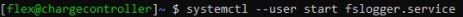
\includegraphics[scale=1.3]{pics/loggerStart.JPG}
    \caption{Logger Programm wird gestartet}
    \label{fig:impl:loggerStart}
\end{figure}

\begin{figure}[h t]
    \centering
    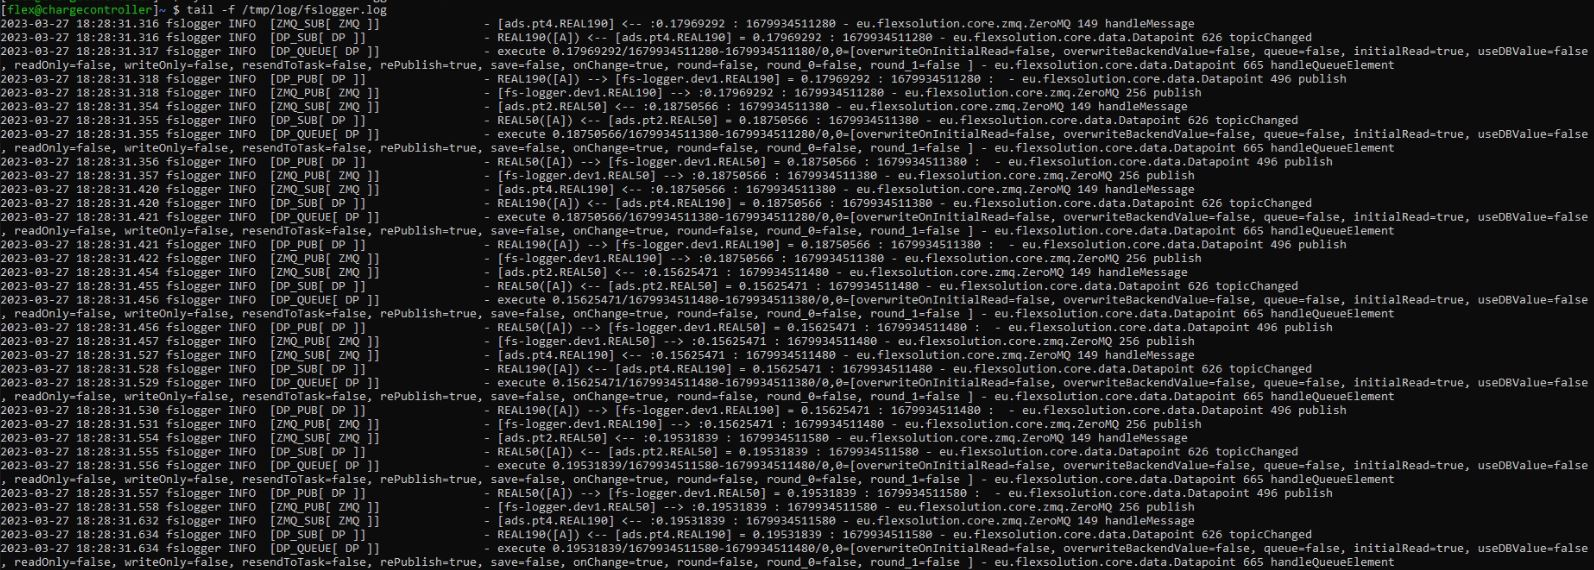
\includegraphics[scale=0.4]{pics/loggerLog.JPG}
    \caption{Ausgabe des Logger Programms}
    \label{fig:impl:loggerLog}
\end{figure}

\begin{figure}[h t]
    \centering
    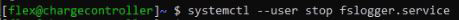
\includegraphics[scale=0.75]{pics/loggerEnd2.JPG}
    \caption{Logger Programm wird gestoppt}
    \label{fig:impl:loggerEnd}
\end{figure}

\subsection{Log4J}
% < 1 https://books.google.at/books?hl=de&lr=&id=hZBimlxiyAcC&oi=fnd&pg=PA9&dq=log4j&ots=QiOna081Z6&sig=9h3lwPqN-rm07kAHln-tLSUfgJY&redir_esc=y#v=onepage&q=log4j&f=false The Complete Log4j Manual, von: Ceki Gülcü S15
% < 1 https://logging.apache.org/log4j/2.x/
Log4J ist ein Framework, um Anwendungsmeldungen von Java zu loggen.
Das Design von Log4J konzentriert sich vor allem darauf, schnell, flexibel und leicht verständlich zu sein. Da Logging eine Applikation verlangsamen kann, wird vor allem ein Wert auf die Schnelligkeit gelegt. \cite{log4JBuch} 

Es ist ein populäres Logging-Package für Java. Logging liefert präzise Informationen über den Ablauf einer Applikation. \cite{log4J}


Anwendungen, welche Log4j verwenden, fordern vom LogManager einen Logger mit einem bestimmten Namen an. Der LogManager sucht den entsprechenden LoggerContext und ruft dann dessen Logger ab. 
Wenn erst ein Logger erstellt werden muss, wird er mit der LoggerConfig verknüpft, die entweder 

\begin{compactitem}
    \item[a)] den gleichen Namen wie der Logger, 
    \item[b)] den Namen eines übergeordneten Pakets oder 
    \item[c)] die Stamm-LoggerConfig enthält.
\end{compactitem}

LoggerConfig-Objekte werden aus Logger-Deklarationen in der Konfiguration erstellt. Die LoggerConfig ist mit den Appendern verbunden, welche die LogEvents tatsächlich liefern, siehe Abb. \ref{fig:impl:log4jArchitektur}. \cite{log4J}

\begin{figure}[h t]
    \centering
    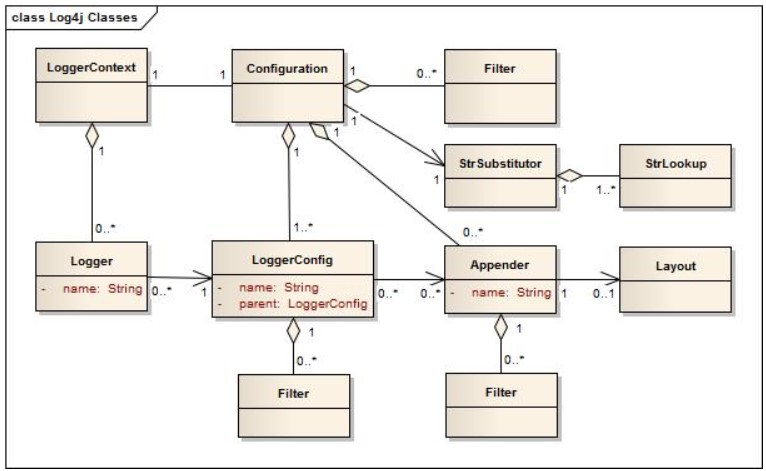
\includegraphics[scale=0.7]{pics/log4jArchitektur.jpg}
    \caption{log4J Architektur \cite{log4J}}
    \label{fig:impl:log4jArchitektur}
\end{figure}

\newpage

\begin{spacing}{1}
    \section{Threads}\label{section:threads}
    \end{spacing}
 
% \subsection{Streams}
 
% \subsection{Lambda}
 
\subsection{Serialisierung (Nebenläufigkeit und Parallelität)}
% 1 Java ist auch eine Insel - Einführung, Ausbildung, Praxis ; von: Christian Ullenboom
Wenn in Java über Nebenläufigkeit gesprochen wird, sind dabei Threads gemeint. Diese sorgen für eine gleichzeitige Abarbeitung von Programmen bzw. der Ressourcen. Dies kann umgesetzt werden, indem die Hardware mehrere Prozessoren oder Kerne besitzt und diese parallel Prozesse abarbeiten können.
 
Bei einem modernen Ein-Prozessor-Betriebssystem wirkt es oft, als wären die Prozesse parallel, doch dies wird einem nur vorgespielt, indem der Prozessor alle paar Sekunden auf einen anderen Prozess wechselt. Bei einem Betriebssystem mit mehreren Kernen, werden die Prozesse wirklich parallel bearbeitet.
 
\subsubsection{Nebenläufigkeit von Programmen steigert Geschwindigkeit}
Wie nebenläufige Abarbeitung die Performance bei einem Einprozessorsystem beschleunigt, kann an folgendem Beispiel-Programm betrachtet werden:
 
\begin{compactitem}
    \item Programm führt eine Reihe von Befehlen aus
    \item Programm soll Datenbank-Report erstellen/visualisieren    
    \item Dabei können einige Prozesse nebenläufig abgearbeitet werden
    \item Diese Prozesse sind zum Beispiel: Öffnen der Datenbank, Lesen neuer Datensätze gleichzeitig mit dem Analysieren alter Daten, alte Daten können in eine Report-Datei geschrieben werden während neue Daten analysiert werden
    \item Wenn diese Prozesse parallel ausgeführt werden, kann sehr viel Zeit eingespart werden beziehungsweise die Performance sehr erhöht werden.
    \item Dieses Beispiel zeigt allerdings auch, dass Nebenläufigkeit sehr gut geplant werden muss.
\end{compactitem}
 
 
\subsection{Concurrency/Gleichzeitigkeit}
% 0 https://www.baeldung.com/java-util-concurrent
% 0 https://reader.elsevier.com/reader/sd/pii/S0167642305000663?token=33C353917B1806AF8A5D40D069D18442FDCF27727ADE08478255219D5D7D6849BA4E8FAE2A474A3FDCD3CC0A36740643&originRegion=eu-west-1&originCreation=20230105151331
% 1 Java ist auch eine Insel - Einführung, Ausbildung, Praxis; von: Christian Ullenboom
Die Ausführung des Programmcodes wird bei einem modernen Betriebssystem von Prozessen, welche jeweils mindestens einen Thread beherbergen, ausgeführt. Das Interessante daran ist, dass nicht etwa die Prozesse nebenläufig ausgeführt werden, sondern die Threads. Dabei können die Threads auf den gleichen Adressraum zugreifen.
 
\subsubsection{Zustände eines Threads}
\begin{compactitem}
    \item Noch nicht erzeugt: Lebenslauf beginnt mit Schlüsselwort \texttt{new}
    \item Running (Laufend) und Not Running (Nicht laufend); Thread kommt in den Zustand Running, wenn die Methode \texttt{run()} aufgerufen wird. Wenn ein anderer Thread den Prozessor des aktuellen Threads übernimmt, kommt der Thread in den Zustand Not Running.    
    \item Waiting (Wartend): Thread befindet sich in einem Wartezustand
    \item Beendet: Aktivität des Threads wurde beendet
\end{compactitem}
 
\subsection{Aufbau eines Threads}
\subsubsection{Interface Runnable}
Dem Thread muss ein Befehlsobjekt des Typs Runnable übergeben werden \ref{lst:impl:javaRunnable}, um wissen zu können, welcher Code ausgeführt werden soll.
Wenn der Thread gestartet wird, werden die Codezeilen im Befehlsobjekt nebenläufig zum anderen Code in dem Programm ab.
 
\begin{lstlisting}[language=java,caption=Java Runnable,label=lst:impl:javaRunnable]
    interface java.lang.Runnable
\end{lstlisting}
 
Durch dieses Interface kann nun die run()-Methode verwendet werden. \ref{lst:impl:threadExample}
 
\begin{lstlisting}[language=java,caption=Einfaches Thread Beispiel,label=lst:impl:threadExample]
    public class CommandThread implements Runnable { 
        @Override public void run() {   
            ...
            }
        }
\end{lstlisting}
 
Dieser Thread kann nun in einer anderen Klasse verwendet werden, indem er zum Beispiel gestartet (\texttt{thread.start()}) oder gestoppt (\texttt{thread.stop()}) wird. \ref{lst:impl:threadStart}
 
\begin{lstlisting}[language=java,caption=Thread erstellen/starten,label=lst:impl:threadStart]
    Thread t1 = new Thread( new CommandThread() );
    t1.start();
\end{lstlisting}
 
Zusätzlich ist es auch noch möglich, den Thread mit (\texttt{thread.sleep(ms)}) zu pausieren.
 
\subsection{BlockingQueue}
% 1 https://jenkov.com/tutorials/java-util-concurrent/blockingqueue.html#java-blockingqueue-tutorial-video
% 0 https://dl.acm.org/doi/pdf/10.1145/3472456.3472458
% 0 blocking queue:  https://books.google.at/books?id=mvzgNSmHEUAC&pg=PT856&dq=java+blocking+queue&hl=de&sa=X&ved=2ahUKEwiF4Jej3bD8AhUNxwIHHcjWBlMQ6AF6BAgEEAI#v=onepage&q=java%20blocking%20queue&f=false
 
Eine BlockingQueue hat typischerweise einen Thread, welcher Objekte produziert und einen anderen, welcher die Objekte konsumiert. \ref{fig:impl:BlockingQueue}
 
\begin{figure}[h t]
    \centering
    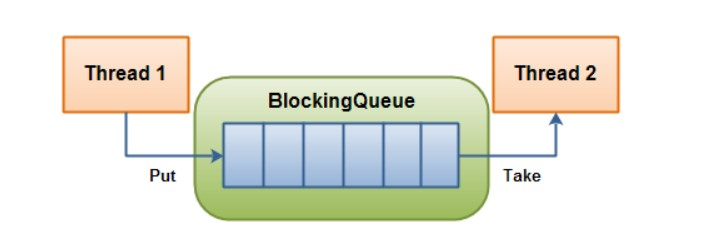
\includegraphics[scale=0.5]{pics/blockingQueue.jpg}
    \caption{Blocking Queue}
    \label{fig:impl:BlockingQueue}
\end{figure}
 
Der produzierende Thread wird weiterhin Objekte produzieren und sie zur BlockingQueue hinzufügen, bis das Limit der Queue erreicht wird. Wenn dieses Limit erreicht wird, wird der Producer-Thread blockiert, während er versucht ein neues Objekt hinzuzufügen. Der Producer Thread bleibt dabei blockiert, bis ein Consumer Thread ein Objekt aus der Queue nimmt.
 
Auf der anderen Seite nimmt der Consumer Thread Objekte aus der Queue, um sie weiter zu verarbeiten. Wenn der Thread versucht ein Objekt aus einer leeren Queue zu nehmen, wird er blockiert, bis der Producer-Thread ein Objekt in die Queue hinzufügt.
 
\subsubsection{BlockingQueue Methoden}
Um die Blocking Queue mit Daten zu bespielen, gibt es spezielle Methoden.
 
\begin{center}
    \begin{tabular}{ |c|c| }
     \hline
     put(o) & fügt Objekte in die BlockingQueue hinzu \\
     \hline
     take() & nimmt Objekte aus der BlockingQueue \\
     \hline
    \end{tabular}
    \end{center}
 
Wenn die Operation bei einer der Methoden erfolglos war, blockiert die Methode, bis die Operation erfolgreich war.
 
\subsubsection{Java Blocking Queue Beispiel}
Das Beispiel unten angeführt verwendet eine ArrayBlockingQueue als Implementation.
 
 
 
\begin{lstlisting}[language=java,caption=Java BlockingQueue Beispiel,label=lst:impl:blockingQueue]
    public class BlockingQueueClass {
    public static void main(String[] args) throws Exception {
        BlockingQueue blockingQueue = new ArrayBlockingQueue(2048);
        Producer producer = new Producer(queue);
        Consumer consumer = new Consumer(queue);
        new Thread(producer).start();
        new Thread(consumer).start();
        Thread.sleep(4000);
    }
    #################################################
 
    public class Producer implements Runnable{
        protected BlockingQueue queue = null;
        public Producer(BlockingQueue queue) {
            this.queue = queue;
        }
        public void run() {
            try {
                queue.put("object1");
                Thread.sleep(1000);
                queue.put("2");
            } catch (InterruptedException e) { e.printStackTrace();}
    }}
    #################################################
    public class Consumer implements Runnable{
        protected BlockingQueue queue = null;
        public Consumer(BlockingQueue queue) {
            this.queue = queue;
        }
        public void run() {
            try {
                System.out.println(queue.take());
                System.out.println(queue.take());
            } catch (InterruptedException e) { e.printStackTrace();}
    }}
}
\end{lstlisting}
 
\subsection{Service executer}
% 0 https://www.baeldung.com/java-executor-service-tutorial
% 1 Java ist auch eine Insel - Einführung, Ausbildung, Praxis; von: Christian Ullenboom
Der Service Executer hilft dabei, den eigentlichen arbeitenden Thread von dem Runnable zu trennen. Denn, wenn ein Thread erzeugt wird, muss das Runnable-Objekt im Konstruktor übergeben werden, dies kann zu Problemen führen, da das Thread-Objekt somit nicht vorher erstellt bzw. aufgebaut werden kann. Ein weiterer Grund, das Runnable und den Thread zu teilen, ist, dass ein Thread nicht einfach so ein anderes Runnable bearbeiten kann, da dieses vorher schon zugewiesen wurde.
 
% \subsection{Java Futures}
% 0 https://www.baeldung.com/java-future
% \subsection{Java Completablefutures}
 
 
% \subsection{First come first serve (Möglichkeiten Prozesse abzuarbeiten)}
 


% \begin{spacing}{1}
%    \section{Performance}\label{section:performance}
%    \end{spacing}
%% https://www.usenix.org/legacy/publications/library/proceedings/neworl/full_papers/seltzer.pdf
% https://cs.brown.edu/courses/cs227/archives/2008/Papers/Compression/GraefeShapiro.pdf
\subsection{Grenzen (Wie viel Daten gleichzeitig kommen können)}
\subsection{Bandbreite}
\subsection{Menge der Datenpunkte}

\begin{spacing}{1}
    \section{Abspeicherung von Daten}\label{section:savedata}
    \end{spacing}
\subsection{Vergleich Vor- und Nachteile JSON vs CSV vs Datenbank}
% 0 https://www.naukri.com/learning/articles/csv-vs-json-for-your-data-science-projects/
% 1 https://www.analyticsinsight.net/csv-or-json-which-format-is-better-for-your-ai-training-data/
Vor allem wenn es darum geht, große Datenmengen abzuspeichern, ist es besonders wichtig, das richtige Datenformat auszuwählen. In diesem Abschnitt wird das CSV, das JSON, und eine herkömmliche Datenbank verglichen. 

Daten können intern oder extern generiert werden und dabei gibt es verschiedene Möglichkeiten, die Daten passend abzuspeichern. Es ist sehr wichtig, das richtige Format auszuwählen, da davon einige Faktoren abhängen. Dazu gehören die Verarbeitungsgeschwindigkeit, sowie die Speichergröße. 
Außerdem kann das Format die Skalierbarkeit, die Kompatibilität, die Cloud-Speicherkosten und die Performance-Geschwindigkeit beeinflussen. 
Konkrete Beispiele, warum bestimmte Dateiformate ausgewählt werden sollten, sind: Geld zu sparen, indem zu einem CSV-Dateiformat gewechselt wird, wenn große Datensets im Cloud-Speicher verarbeitet werden. JSON ist eine bessere Wahl, wenn es darum geht, kleinere Datensets mit einer komplexen Hierarchie zu speichern. 
Im Allgemeinen bedeutet dies, dass das richtige Datenformat Geld und Zeit spart.  

\begin{center}
    \begin{tabular}{ |c|c|c|c| } 
     \hline
     \multicolumn{4}{|c|}{Ein genauerer Vergleich (exaktere Daten kommen noch) } \\
     \hline
     \hline
     Features & CSV & JSON & Datenbank \\ 
     \hline 
     \hline
     Speicheranforderung & weniger Platz & mehr Platz & ? \\ 
     \hline
     Verarbeitungsgeschwindigkeit & schnell & langsam & ? \\ 
     \hline
     Security & sicherer & unsicherer & sicherer \\ 
     \hline
     Große oder komplexe Datensets & große Datensets & komplexe Datensets & Beides \\ 
     \hline
    \end{tabular}
    \end{center}

\subsection{CSV}
CSV ist ein Text-Dateiformat, mit der Besonderheit, dass die Werte durch Semikolons unterteilt werden. Dadurch eignet es sich sehr gut für eine Speicherung von sehr vielen Daten. Jede Reihe der CSV-Datei repräsentiert dabei eine Zeile von Daten, die Spalten werden dabei von den Strichpunkten unterteilt. Das CSV-Format kann die Nutzung von Speicherplatz, sowie das Austauschen von Daten maximieren. Strukturierte CSV-Files können außerdem einen Header enthalten, welcher jede Spalte einordnet. CSV-Dateien können außerdem nicht nur durch Semikolons, sondern auch durch Kommas, Tabs und Abstände unterteilt werden. CSV wird am meisten in Entwicklungseinrichtungen und technischen Konsumenten-Anwendungen verwendet. Ein weiterer Vorteil von dem CSV-Dateiformat ist, dass es von der meisten Datenverarbeitungs-Software importiert, konvertiert und exportiert werden kann. Mithilfe dieser Softwares kann die CSV-Dateien auch sehr einfach serialisiert oder deserialisiert werden. CSV ist ein sehr einfach aufgebautes Format und kann somit von fast jedem Datenanalysator ausgewertet werden. Als Nachteile von CSV kann aufgezählt werden, dass es im Rohformat schwer zu lesen ist, und es anfällig für menschliche Fehler ist. Der größte Nachteil gegenüber den anderen zwei Datenformaten sind auf jeden Fall die limitierten Möglichkeiten, die Daten komplex aufzubereiten.   


\subsection{JSON}
JSON ist im Vergleich zu CSV leichter verständlich für Menschen. Die Daten werden als semi-strukturiert angezeigt. \ref{lst:impl:json} JSON ist sehr weit kompatibel und wird somit von vielen Software-Entwicklern verwendet, um configs und APIs zu designen. Da JSON von JavaScript entwickelt wurde, kann es sehr einfach in eine Java-basierte Umgebung integriert werden. Somit wird JSON sehr oft für die Datenverarbeitung von Front- und Backend verwendet. Mithilfe von JSON kann sehr einfach auf neue Daten zugegriffen werden. Gerade wenn es um rationales und hierarchisches Datenmanagement geht, eignet sich JSON sehr gut, da es dies sehr unterstützt. JSON-Dateien sind selbsterklärend und es ist für Systeme sehr leicht, eine JSON-Datei zu erkennen und zu verarbeiten. JSON ist somit auch sehr viel einfacher zu lesen als CSV-Dateien. 


\begin{lstlisting}[language=java,caption=JSON Beispiel,label=lst:impl:json]
    {   "pupil": {
            "id":       "1"
            "name":     "Margaret"
        }
    }
\end{lstlisting}

\subsection{Datenbank}
